The purpose of the VRGP is to provide a standardized way of communication for vessels and Maritime Operating Centres (MOC) on the shore. Most importantly, VRGP includes streaming live data from the vessel to the shore and, based on this data, sending guidance messages from the shore to the vessel. This system, a VRGP implementation for the Åboat and, therefore, a maritime system, serves as a proof of concept of the protocol specification and standardizes the external communication of the Åboat.
\\\\
The VRGP implementation will provide the Åboat with the functionality described in the protocol specification, an interface for communication with a MOC. This includes initiating and creating a connection with a MOC, streaming on-board information upon request, terminating a connection, sending notification about abnormal situations on board and receiving guidance from the MOC. The VRGP implementation will be integrated into the existing Åboat architecture and connect with its user interface.
\\\\
The implementation can also be used as a starting point for other implementations. Parts of it will be reusable and the core implementation may even be an independent component to be used by other vessels than the Åboat.

\section{Functional Requirements}\label{sec:func-requirements}

\begin{figure}[ht]
	\centering
	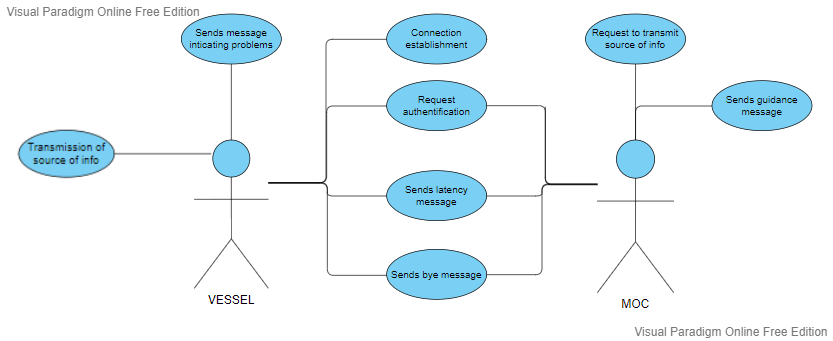
\includegraphics[width=\linewidth]{diagrams/use-case-diagram}
	\caption{Use case diagram}
	\label{fig:use-case-diagram}
\end{figure}

\subsection{Initiate Connection}

\begin{table}[H]
	\centering
	\begin{tabularx}{\textwidth}{ l X }
		\rowcolor[HTML]{E7E7E7}
		\textbf{ID} & F-REQ-1 \\
		\textbf{Description} & The VRGP implementation MUST provide tools for the vessel to connect to a MOC at any given moment. \\
		\rowcolor[HTML]{E7E7E7}
		\textbf{Priority} & \priohigh \\
		\textbf{Dependencies} & Specialized by F-REQ-1.1, F-REQ-1.2 \\
		\rowcolor[HTML]{E7E7E7}
		\textbf{Input/trigger} & The vessel wants to establish a connection with an MOC. \\
		\textbf{Output} & A connection is established. \\
		\rowcolor[HTML]{E7E7E7}
		\textbf{Actors} & Vessel, MOC \\
	\end{tabularx}
	\label{table:f-req-1}
\end{table}

\begin{table}[H]
\centering
	\begin{tabularx}{\textwidth}{ l X }
		\rowcolor[HTML]{E7E7E7}
		\textbf{ID} & F-REQ-1.1 \\
		\textbf{Description} & The second message at the start of every connection or the message after authentication MUST be one of a vessel type, which is a message that specifies information of the vessel. \\
		\rowcolor[HTML]{E7E7E7}
		\textbf{Priority} & \priohigh \\
		\textbf{Dependencies} & Specializes F-REQ-1 \\
		\rowcolor[HTML]{E7E7E7}
		\textbf{Input/trigger} & Vessel message indicating the vessel’s capabilities. \\
		\textbf{Output} & Acknowledgment from the MOC. \\
		\rowcolor[HTML]{E7E7E7}
		\textbf{Actors} & Vessel, MOC \\
	\end{tabularx}
	\label{table:f-req-1.1}
\end{table}

\begin{table}[H]
	\centering
	\begin{tabularx}{\textwidth}{ l X }
		\rowcolor[HTML]{E7E7E7}
		\textbf{ID} & F-REQ-1.2 \\
		\textbf{Description} & The VRGP implementation MUST provide an interface for other modules to establish new connections.  \\
		\rowcolor[HTML]{E7E7E7}
		\textbf{Priority} & \priohigh \\
		\textbf{Dependencies} & Specializes F-REQ-1 \\
		\rowcolor[HTML]{E7E7E7}
		\textbf{Input/trigger} & A software module of a vessel wants to establish a new connection. \\
		\textbf{Output} & A connection is established through the VRGP implementation interface. \\
		\rowcolor[HTML]{E7E7E7}
		\textbf{Actors} & Vessel, MOC \\
	\end{tabularx}
	\label{table:f-req-1.2}
\end{table}

\begin{table}[H]
	\centering
	\begin{tabularx}{\textwidth}{ l X }
		\rowcolor[HTML]{E7E7E7}
		\textbf{ID} & F-REQ-1.2.1 \\
		\textbf{Description} & The connection initiation interface SHOULD be used for autonomous access and by the Åboat user interface. \\
		\rowcolor[HTML]{E7E7E7}
		\textbf{Priority} & \priohigh \\
		\textbf{Dependencies} & Specializes F-REQ-1.2 \\
		\rowcolor[HTML]{E7E7E7}
		\textbf{Input/trigger} & A software module of a vessel wants to establish a new connection. \\
		\textbf{Output} & A connection is established through the VRGP implementation interface. \\
		\rowcolor[HTML]{E7E7E7}
		\textbf{Actors} & Vessel, MOC \\
	\end{tabularx}
	\label{table:f-req-1.2.1}
\end{table}

\subsection{Information Streams}

\begin{table}[H]
	\centering
	\begin{tabularx}{\textwidth}{ l X }
		\rowcolor[HTML]{E7E7E7}
		\textbf{ID} & F-REQ-2 \\
		\textbf{Description} & MOC can request the vessel to transmit any available or supported source of information on board. \\
		\rowcolor[HTML]{E7E7E7}
		\textbf{Priority} & \priohigh \\
		\textbf{Dependencies} & Depends on F-REQ-4.1 \\
		\rowcolor[HTML]{E7E7E7}
		\textbf{Input/trigger} & The MOC asks the vessel to show one or more sources of information on board. \\
		\textbf{Output} & The vessel responds with relevant information. \\
		\rowcolor[HTML]{E7E7E7}
		\textbf{Actors} & Vessel, MOC \\
	\end{tabularx}
	\label{table:f-req-2}
\end{table}

\begin{table}[H]
	\centering
	\begin{tabularx}{\textwidth}{ l X }
		\rowcolor[HTML]{E7E7E7}
		\textbf{ID} & F-REQ-2.1 \\
		\textbf{Description} & The vessel MUST transmit the video stream upon request by a MOC. \\
		\rowcolor[HTML]{E7E7E7}
		\textbf{Priority} & \priohigh \\
		\textbf{Dependencies} & Depends on F-REQ-4.1 \\
		\rowcolor[HTML]{E7E7E7}
		\textbf{Input/trigger} & The MOC asks the vessel to transmit video streams from its cameras. \\
		\textbf{Output} & The vessel responds with the relevant video streams. \\
		\rowcolor[HTML]{E7E7E7}
		\textbf{Actors} & Vessel, MOC \\
	\end{tabularx}
	\label{table:f-req-2.1}
\end{table}

\begin{table}[H]
	\centering
	\begin{tabularx}{\textwidth}{ l X }
		\rowcolor[HTML]{E7E7E7}
		\textbf{ID} & F-REQ-2.2 \\
		\textbf{Description} & The vessel MUST transmit the position data upon request by a MOC. \\
		\rowcolor[HTML]{E7E7E7}
		\textbf{Priority} & \priohigh \\
		\textbf{Dependencies} & Depends on F-REQ-4.1 \\
		\rowcolor[HTML]{E7E7E7}
		\textbf{Input/trigger} & The MOC asks the vessel to transmit the position data from the GPS. \\
		\textbf{Output} & The vessel starts sharing the position data from the GPS. \\
		\rowcolor[HTML]{E7E7E7}
		\textbf{Actors} & Vessel, MOC \\
	\end{tabularx}
	\label{table:f-req-2.2}
\end{table}

\begin{table}[H]
	\centering
	\begin{tabularx}{\textwidth}{ l X }
		\rowcolor[HTML]{E7E7E7}
		\textbf{ID} & F-REQ-2.3 \\
		\textbf{Description} & The vessel MUST transmit the directional data upon request by a MOC. \\
		\rowcolor[HTML]{E7E7E7}
		\textbf{Priority} & \priohigh \\
		\textbf{Dependencies} & Depends on F-REQ-4.1 \\
		\rowcolor[HTML]{E7E7E7}
		\textbf{Input/trigger} & The MOC asks the vessel to transmit directional data from the compass. \\
		\textbf{Output} & Vessel starts transmitting the requested data. \\
		\rowcolor[HTML]{E7E7E7}
		\textbf{Actors} & Vessel, MOC \\
	\end{tabularx}
	\label{table:f-req-2.3}
\end{table}

\begin{table}[H]
	\centering
	\begin{tabularx}{\textwidth}{ l X }
		\rowcolor[HTML]{E7E7E7}
		\textbf{ID} & F-REQ-2.4 \\
		\textbf{Description} & The vessel MUST transmit the heading data upon request by a MOC. \\
		\rowcolor[HTML]{E7E7E7}
		\textbf{Priority} & \priohigh \\
		\textbf{Dependencies} & Depends on F-REQ-4.1 \\
		\rowcolor[HTML]{E7E7E7}
		\textbf{Input/trigger} & The MOC asks the vessel to transmit the heading from the motor. \\
		\textbf{Output} & Vessel starts sharing the heading from the motor. \\
		\rowcolor[HTML]{E7E7E7}
		\textbf{Actors} & Vessel, MOC \\
	\end{tabularx}
	\label{table:f-req-2.4}
\end{table}

\begin{table}[H]
	\centering
	\begin{tabularx}{\textwidth}{ l X }
		\rowcolor[HTML]{E7E7E7}
		\textbf{ID} & F-REQ-2.5 \\
		\textbf{Description} & The vessel MUST transmit the speed data upon request by a MOC. \\
		\rowcolor[HTML]{E7E7E7}
		\textbf{Priority} & \priohigh \\
		\textbf{Dependencies} & Depends on F-REQ-4.1 \\
		\rowcolor[HTML]{E7E7E7}
		\textbf{Input/trigger} & The MOC asks the vessel to transmit the speed from the motor. \\
		\textbf{Output} & Vessel starts sharing the speed from the motor. \\
		\rowcolor[HTML]{E7E7E7}
		\textbf{Actors} & Vessel, MOC \\
	\end{tabularx}
	\label{table:f-req-2.5}
\end{table}

\begin{table}[H]
	\centering
	\begin{tabularx}{\textwidth}{ l X }
		\rowcolor[HTML]{E7E7E7}
		\textbf{ID} & F-REQ-2.6 \\
		\textbf{Description} & The vessel MUST transmit the rate of turn upon request by a MOC. \\
		\rowcolor[HTML]{E7E7E7}
		\textbf{Priority} & \priohigh \\
		\textbf{Dependencies} & Depends on F-REQ-4.1 \\
		\rowcolor[HTML]{E7E7E7}
		\textbf{Input/trigger} & The MOC asks the vessel to transmit the rate of turn from the motor. \\
		\textbf{Output} & Vessel starts sharing the speed from the motor. \\
		\rowcolor[HTML]{E7E7E7}
		\textbf{Actors} & Vessel, MOC \\
	\end{tabularx}
	\label{table:f-req-2.6}
\end{table}

\begin{table}[H]
	\centering
	\begin{tabularx}{\textwidth}{ l X }
		\rowcolor[HTML]{E7E7E7}
		\textbf{ID} & F-REQ-2.7 \\
		\textbf{Description} & The vessel MUST transmit the Lidar data upon request by a MOC. \\
		\rowcolor[HTML]{E7E7E7}
		\textbf{Priority} & \priohigh \\
		\textbf{Dependencies} & Depends on F-REQ-4.1 \\
		\rowcolor[HTML]{E7E7E7}
		\textbf{Input/trigger} & The MOC asks the vessel to transmit Lidar data. \\
		\textbf{Output} & The vessel starts transmitting the requested data. \\
		\rowcolor[HTML]{E7E7E7}
		\textbf{Actors} & Vessel, MOC \\
	\end{tabularx}
	\label{table:f-req-2.7}
\end{table}

\begin{table}[H]
	\centering
	\begin{tabularx}{\textwidth}{ l X }
		\rowcolor[HTML]{E7E7E7}
		\textbf{ID} & F-REQ-2.8 \\
		\textbf{Description} & The vessel MAY transmit internal data upon request by a MOC. \\
		\rowcolor[HTML]{E7E7E7}
		\textbf{Priority} & \prioopt \\
		\textbf{Dependencies} & Depends on F-REQ-4.1 \\
		\rowcolor[HTML]{E7E7E7}
		\textbf{Input/trigger} & The MOC asks the vessel to transmit inertial data. \\
		\textbf{Output} & Vessel  starts transmitting the requested data. \\
		\rowcolor[HTML]{E7E7E7}
		\textbf{Actors} & Vessel, MOC \\
	\end{tabularx}
	\label{table:f-req-2.8}
\end{table}

\subsection{Terminate Connection}

\begin{table}[H]
	\centering
	\begin{tabularx}{\textwidth}{ l X }
		\rowcolor[HTML]{E7E7E7}
		\textbf{ID} & F-REQ-3 \\
		\textbf{Description} & Vessel and MOC can decide to end the communication at any point. \\
		\rowcolor[HTML]{E7E7E7}
		\textbf{Priority} & \priohigh \\
		\textbf{Dependencies} & Depends on F-REQ-1 \\
		\rowcolor[HTML]{E7E7E7}
		\textbf{Input/trigger} & One of the actors sends a “bye” message to end the communication at any point. \\
		\textbf{Output} & The communication ends. \\
		\rowcolor[HTML]{E7E7E7}
		\textbf{Actors} & Vessel, MOC \\
	\end{tabularx}
	\label{table:f-req-3}
\end{table}

\begin{table}[H]
	\centering
	\begin{tabularx}{\textwidth}{ l X }
		\rowcolor[HTML]{E7E7E7}
		\textbf{ID} & F-REQ-3.1 \\
		\textbf{Description} & The vessel MUST be able to end the communication by sending a closing message. \\
		\rowcolor[HTML]{E7E7E7}
		\textbf{Priority} & \priohigh \\
		\textbf{Dependencies} & Depends on F-REQ-3 \\
		\rowcolor[HTML]{E7E7E7}
		\textbf{Input/trigger} & The vessel can send a message to end the communication at any point. \\
		\textbf{Output} & The communication ends. \\
		\rowcolor[HTML]{E7E7E7}
		\textbf{Actors} & Vessel, MOC \\
	\end{tabularx}
	\label{table:f-req-3.1}
\end{table}

\begin{table}[H]
	\centering
	\begin{tabularx}{\textwidth}{ l X }
		\rowcolor[HTML]{E7E7E7}
		\textbf{ID} & F-REQ-3.2 \\
		\textbf{Description} & The MOC MUST be able to end the communication by sending a closing message \\
		\rowcolor[HTML]{E7E7E7}
		\textbf{Priority} & \priohigh \\
		\textbf{Dependencies} & Depends on F-REQ-3 \\
		\rowcolor[HTML]{E7E7E7}
		\textbf{Input/trigger} & The MOC can send a message to end the communication at any point. \\
		\textbf{Output} & The communication ends. \\
		\rowcolor[HTML]{E7E7E7}
		\textbf{Actors} & Vessel, MOC \\
	\end{tabularx}
	\label{table:f-req-3.2}
\end{table}

\begin{table}[H]		
	\centering
	\begin{tabularx}{\textwidth}{ l X }
		\rowcolor[HTML]{E7E7E7}
		\textbf{ID} & F-REQ-3.3 \\
		\textbf{Description} & The VRGP implementation MUST provide an interface for other modules to end connections. \\
		\rowcolor[HTML]{E7E7E7}
		\textbf{Priority} & \priohigh \\
		\textbf{Dependencies} & Depends on F-REQ-1, specialized by F-REQ-3.3.1 \\
		\rowcolor[HTML]{E7E7E7}
		\textbf{Input/trigger} & A software module of a vessel wants to establish a new connection. \\
		\textbf{Output} & A connection is established through the VRGP implementation interface. \\
		\rowcolor[HTML]{E7E7E7}
		\textbf{Actors} & Vessel, MOC \\
	\end{tabularx}
	\label{table:f-req-3.3}
\end{table}

\begin{table}[H]
	\centering
	\begin{tabularx}{\textwidth}{ l X }
		\rowcolor[HTML]{E7E7E7}
		\textbf{ID} & F-REQ-3.3.1 \\
		\textbf{Description} & The connection termination interface SHOULD be used for autonomous access and by the Åboat user interface. \\
		\rowcolor[HTML]{E7E7E7}
		\textbf{Priority} & \priohigh \\
		\textbf{Dependencies} & Specializes F-REQ-3.3 \\
		\rowcolor[HTML]{E7E7E7}
		\textbf{Input/trigger} & A software module of a vessel wants to establish a new connection \\
		\textbf{Output} & A connection is established through the VRGP implementation interface that is used via the UI. \\
		\rowcolor[HTML]{E7E7E7}
		\textbf{Actors} & Vessel, MOC \\
	\end{tabularx}
	\label{table:f-req-3.3.1}
\end{table}

\subsection{Authentication}

\begin{table}[H]
	\centering
	\begin{tabularx}{\textwidth}{ l X }
		\rowcolor[HTML]{E7E7E7}
		\textbf{ID} & F-REQ-4.1 \\
		\textbf{Description} & The VRGP implementation MUST support certificate authentication:
			\begin{itemize}
				\item Certificates MUST always be provided by trustworthy authorities.
				\item Either party can request authentication.
				\item Typically, a vessel SHOULD request authentication from the MOC and the MOC SHOULD respond with an authentication certificate.
				\item Precondition: MOC and vessels need to be registered in the Maritime Identity Connectivity Platform.
				\item The implementation SHOULD provide authentication error handling if the party cannot, or does not wish to participate in the authentication exchange.
			\end{itemize} \\
		\rowcolor[HTML]{E7E7E7}
		\textbf{Priority} & \priohigh \\
		\textbf{Dependencies} & specializes F-REQ-10, depends on F-REQ-1.1 \\
		\rowcolor[HTML]{E7E7E7}
		\textbf{Input/trigger} & An authentication certificate issued by the MCP. \\
		\textbf{Output} & Other party’s certificate issued by the MCP. \\
		\rowcolor[HTML]{E7E7E7}
		\textbf{Actors} & Vessel, MOC \\
	\end{tabularx}
	\label{table:f-req-4.1}
\end{table}

\begin{table}[H]
	\centering
	\begin{tabularx}{\textwidth}{ l X }
		\rowcolor[HTML]{E7E7E7}
		\textbf{ID} & F-REQ-4.2 \\
		\textbf{Description} & The protocol MAY supports token authentication to allow the vessel-side crew to authenticate using their account credentials. \\
		\rowcolor[HTML]{E7E7E7}
		\textbf{Priority} & \prioopt\\
		\textbf{Dependencies} & Specializes NF-REQ-10 \\
		\rowcolor[HTML]{E7E7E7}
		\textbf{Input/trigger} & Username and password \\
		\textbf{Output} & Receives an OIDC token. \\
		\rowcolor[HTML]{E7E7E7}
		\textbf{Actors} & Vessel crew, authentication server \\
	\end{tabularx}
	\label{table:f-req-4.2}
\end{table}

\subsection{Messages about problems on board}

\begin{table}[H]
	\centering
	\begin{tabularx}{\textwidth}{ l X }
		\rowcolor[HTML]{E7E7E7}
		\textbf{ID} & F-REQ-5 \\
		\textbf{Description} & The VRGP implementation SHOULD handle abnormal situations aboard the vessel by sending relevant messages to the MOC. The six levels of severity defined in the protocol that reflect such abnormal situations are: debug, info, caution, warning, alarm, emergency.
			\begin{itemize}
				\item Different levels of severity answer to the gravity of the situation.
				\item The alarms should be implemented to conform to standard IMO-A2021.
			\end{itemize} \\
		\rowcolor[HTML]{E7E7E7}
		\textbf{Priority} & \priohigh \\
		\textbf{Dependencies} & Specialized by F-REQ-5.1, F-REQ-5.2, F-REQ-5.3, F-REQ-5.4, F-REQ-5.5, F-REQ-5.6 \\
		\rowcolor[HTML]{E7E7E7}
		\textbf{Input/trigger} & The vessel sends a notification message with one of the six levels of severity to the MOC. \\
		\textbf{Output} & The MOC should acknowledge the notification message. \\
		\rowcolor[HTML]{E7E7E7}
		\textbf{Actors} & Vessel, MOC \\
	\end{tabularx}
	\label{table:f-req-5}
\end{table}

\begin{table}[H]
	\centering
	\begin{tabularx}{\textwidth}{ l X }
		\rowcolor[HTML]{E7E7E7}
		\textbf{ID} & F-REQ-5.1 \\
		\textbf{Description} & The implementation of the protocol SHOULD provide a “debug” message.
		\begin{itemize}
			\item The debug message is used to convey information that aids the development of the implementation.
			\item This message should not be sent by implementations in actual operational use.
			\item The message must contain relevant information.
		\end{itemize} \\
		\rowcolor[HTML]{E7E7E7}
		\textbf{Priority} & \priohigh \\
		\textbf{Dependencies} & Specializes F-REQ-5 \\
		\rowcolor[HTML]{E7E7E7}
		\textbf{Input/trigger} & The vessel sends a debug message to the MOC. \\
		\textbf{Output} & The MOC should acknowledge the debug message. \\
		\rowcolor[HTML]{E7E7E7}
		\textbf{Actors} & Vessel, MOC \\
	\end{tabularx}
	\label{table:f-req-5.1}
\end{table}

\begin{table}[H]
	\centering
	\begin{tabularx}{\textwidth}{ l X }
		\rowcolor[HTML]{E7E7E7}
		\textbf{ID} & F-REQ-5.2 \\
		\textbf{Description} & The implementation of the protocol SHOULD provide an “info” message.
		\begin{itemize}
			\item The info message is used to convey information that might be useful to the MOC but is not deemed important or critical.
			\item The message must contain relevant information.
		\end{itemize} \\
		\rowcolor[HTML]{E7E7E7}
		\textbf{Priority} & \priohigh \\
		\textbf{Dependencies} & Specializes F-REQ-5 \\
		\rowcolor[HTML]{E7E7E7}
		\textbf{Input/trigger} & The vessel sends an info message to the MOC. \\
		\textbf{Output} & The MOC should acknowledge the info message \\
		\rowcolor[HTML]{E7E7E7}
		\textbf{Actors} & Vessel, MOC \\
	\end{tabularx}
	\label{table:f-req-5.2}
\end{table}

\begin{table}[H]
	\centering
	\begin{tabularx}{\textwidth}{ l X }
		\rowcolor[HTML]{E7E7E7}
		\textbf{ID} & F-REQ-5.3 \\
		\textbf{Description} & The implementation of the protocol SHOULD provide a “caution” message.
		\begin{itemize}
			\item The caution message is used to convey information about a situation or possible issue that the MOC should take note of, is likely to require attention but does not (yet) warrant a warning or alarm.
			\item A caution message should have a relevant category as described by the specification and should reflect the situation on the vessel accurately.
		\end{itemize} \\
		\rowcolor[HTML]{E7E7E7}
		\textbf{Priority} & \priohigh \\
		\textbf{Dependencies} & Specializes F-REQ-5 \\
		\rowcolor[HTML]{E7E7E7}
		\textbf{Input/trigger} & The vessel sends a caution message to the MOC. \\
		\textbf{Output} & The MOC should acknowledge the caution message. \\
		\rowcolor[HTML]{E7E7E7}
		\textbf{Actors} & Vessel, MOC \\
	\end{tabularx}
	\label{table:f-req-5.3}
\end{table}

\begin{table}[H]
	\centering
	\begin{tabularx}{\textwidth}{ l X }
		\rowcolor[HTML]{E7E7E7}
		\textbf{ID} & F-REQ-5.4 \\
		\textbf{Description} & The implementation of the protocol SHOULD provide a “warning” message.
		\begin{itemize}
			\item The warning message is used to convey information about a situation that requires attention.
			\item A warning message should have a relevant category as described by the specification and should reflect the situation on the vessel accurately.
		\end{itemize} \\
		\rowcolor[HTML]{E7E7E7}
		\textbf{Priority} & \priohigh \\
		\textbf{Dependencies} & Specializes F-REQ-5 \\
		\rowcolor[HTML]{E7E7E7}
		\textbf{Input/trigger} & The vessel sends a warning message to the MOC. \\
		\textbf{Output} & The MOC should acknowledge the warning message \\
		\rowcolor[HTML]{E7E7E7}
		\textbf{Actors} & Vessel, MOC \\
	\end{tabularx}
	\label{table:f-req-5.4}
\end{table}

\begin{table}[H]
	\centering
	\begin{tabularx}{\textwidth}{ l X }
		\rowcolor[HTML]{E7E7E7}
		\textbf{ID} & F-REQ-5.5 \\
		\textbf{Description} & The implementation of the protocol SHOULD provide an “alarm” message.
		\begin{itemize}
			\item The alarm message is used to convey information about a situation that requires immediate attention.
			\item An alarm message should have a relevant category as described by the specification and should reflect the situation on the vessel accurately.
		\end{itemize} \\
		\rowcolor[HTML]{E7E7E7}
		\textbf{Priority} & \priohigh \\
		\textbf{Dependencies} & Specializes F-REQ-5 \\
		\rowcolor[HTML]{E7E7E7}
		\textbf{Input/trigger} & The vessel sends an alarm message to the MOC. \\
		\textbf{Output} & The MOC should acknowledge the alarm message. \\
		\rowcolor[HTML]{E7E7E7}
		\textbf{Actors} & Vessel, MOC \\
	\end{tabularx}
	\label{table:f-req-5.5}
\end{table}

\begin{table}[H]
	\centering
	\begin{tabularx}{\textwidth}{ l X }
		\rowcolor[HTML]{E7E7E7}
		\textbf{ID} & F-REQ-5.6 \\
		\textbf{Description} & The implementation of the protocol SHOULD provide an “emergency” message.
		\begin{itemize}
			\item The emergency message is used to convey information about a situation where life or vessel are in immediate danger.
			\item An emergency message should have a relevant category as described by the specification and should reflect the situation on the vessel accurately.
		\end{itemize} \\
		\rowcolor[HTML]{E7E7E7}
		\textbf{Priority} & \priohigh \\
		\textbf{Dependencies} & Specializes F-REQ-5 \\
		\rowcolor[HTML]{E7E7E7}
		\textbf{Input/trigger} & The vessel sends an emergency message to the MOC. \\
		\textbf{Output} & The MOC acknowledges the emergency message. \\
		\rowcolor[HTML]{E7E7E7}
		\textbf{Actors} & Vessel, MOC \\
	\end{tabularx}
	\label{table:f-req-5.6}
\end{table}

\subsection{Latency}

\begin{table}[H]
	\centering
	\begin{tabularx}{\textwidth}{ l X }
		\rowcolor[HTML]{E7E7E7}
		\textbf{ID} & F-REQ-6 \\
		\textbf{Description} & MOCs and vessels can exchange time messages in order to determine latency. \\
		\rowcolor[HTML]{E7E7E7}
		\textbf{Priority} & \priohigh \\
		\textbf{Dependencies} & Depends on F-REQ-7 \\
		\rowcolor[HTML]{E7E7E7}
		\textbf{Input/trigger} & A time message from one party \\
		\textbf{Output} & A time message response from the other party \\
		\rowcolor[HTML]{E7E7E7}
		\textbf{Actors} & Vessel, MOC \\
	\end{tabularx}
	\label{table:f-req-6}
\end{table}

\subsection{Clock synchronisation}

\begin{table}[H]
	\centering
	\begin{tabularx}{\textwidth}{ l X }
		\rowcolor[HTML]{E7E7E7}
		\textbf{ID} & F-REQ-7 \\
		\textbf{Description} & The vessel SHOULD synchronize its clocks (of the systems involved) to a high precision source such as a GNSS or similar service. \\
		\rowcolor[HTML]{E7E7E7}
		\textbf{Priority} & \prioavg \\
		\textbf{Dependencies} & - \\
		\rowcolor[HTML]{E7E7E7}
		\textbf{Input/trigger} & MOC message/connection \\
		\textbf{Output} & A synchronized clock \\
		\rowcolor[HTML]{E7E7E7}
		\textbf{Actors} & Vessel \\
	\end{tabularx}
	\label{table:f-req-7}
\end{table}

\subsection{Guidance}

\todo{Add requirements for guidance.}

\section{User Interface Requirements}\label{sec:ui-requirements}

\begin{table}[H]
	\centering
	\begin{tabularx}{\textwidth}{ l X }
		\rowcolor[HTML]{E7E7E7}
		\textbf{ID} & UI-REQ-9 \\
		\textbf{Description} & The VRGP implementation SHOULD connect to the existing Åboat user interface. \\
		\rowcolor[HTML]{E7E7E7}
		\textbf{Priority} & \prioavg \\
		\textbf{Dependencies} & Depends on REQ-2 \\
		\rowcolor[HTML]{E7E7E7}
		\textbf{Input/trigger} & The user navigates to a page in the user interface that uses data from the VRGP information stream. \\
		\textbf{Output} & The data is displayed \\
		\rowcolor[HTML]{E7E7E7}
		\textbf{Actors} & Åboat UI \\
	\end{tabularx}
	\label{table:ui-req-9}
\end{table}

\begin{table}[H]
	\centering
	\begin{tabularx}{\textwidth}{ l X }
		\rowcolor[HTML]{E7E7E7}
		\textbf{ID} & UI-REQ-9.1 \\
		\textbf{Description} & An extra user interface SHOULD be created for a mock of a MOC including rudimentary implementations of all major MOC operations defined in the protocol specification. A starting point for such a user interface implementation already exists. \\
		\rowcolor[HTML]{E7E7E7}
		\textbf{Priority} & \priolow \\
		\textbf{Dependencies} & - \\
		\rowcolor[HTML]{E7E7E7}
		\textbf{Input/trigger} & - \\
		\textbf{Output} & - \\
		\rowcolor[HTML]{E7E7E7}
		\textbf{Actors} & MOC \\
	\end{tabularx}
	\label{table:ui-req-9.1}
\end{table}

\begin{table}[H]
	\centering
	\begin{tabularx}{\textwidth}{ l X }
		\rowcolor[HTML]{E7E7E7}
		\textbf{ID} & UI-REQ-9.1.1 \\
		\textbf{Description} & The MOC user interface SHOULD include a view with all currently connected vessels. \\
		\rowcolor[HTML]{E7E7E7}
		\textbf{Priority} & \priolow \\
		\textbf{Dependencies} & Specializes UI-REQ-9.1 \\
		\rowcolor[HTML]{E7E7E7}
		\textbf{Input/trigger} & User interface input \\
		\textbf{Output} & User interface output \\
		\rowcolor[HTML]{E7E7E7}
		\textbf{Actors} & MOC \\
	\end{tabularx}
	\label{table:ui-req-9.1.1}
\end{table}

\begin{table}[H]
	\centering
	\begin{tabularx}{\textwidth}{ l X }
		\rowcolor[HTML]{E7E7E7}
		\textbf{ID} & UI-REQ-9.1.2 \\
		\textbf{Description} & The MOC user interface SHOULD include a view for each currently connected vessel with the following contents:
			\begin{itemize}
				\item The current latency
				\item The current conning
				\item Received messages about abnormal situations
				\item The option to request further information and display of requested information
				\item The option to end communication with this vessel
			\end{itemize} \\
		\rowcolor[HTML]{E7E7E7}
		\textbf{Priority} & \priolow \\
		\textbf{Dependencies} & Specializes UI-REQ-9.1 \\
		\rowcolor[HTML]{E7E7E7}
		\textbf{Input/trigger} & User interface input \\
		\textbf{Output} & User interface output \\
		\rowcolor[HTML]{E7E7E7}
		\textbf{Actors} & MOC \\
	\end{tabularx}
	\label{table:ui-req-9.1.2}
\end{table}

\section{Non-functional Requirements}\label{sec:non-func-requirements}

\subsection{Deliverable}

\begin{table}[H]
	\centering
	\begin{tabularx}{\textwidth}{ l X }
		\rowcolor[HTML]{E7E7E7}
		\textbf{ID} & NF-REQ-8 \\
		\textbf{Description} & The software MUST be delivered as an OpenDLV microservice in a Docker container. \\
		\rowcolor[HTML]{E7E7E7}
		\textbf{Priority} & \priohigh \\
		\textbf{Dependencies} & - \\
		\rowcolor[HTML]{E7E7E7}
		\textbf{Actors} & Åboat \\
	\end{tabularx}
	\label{table:nf-req-8}
\end{table}

\subsection{Security}

\begin{table}[H]
	\centering
	\begin{tabularx}{\textwidth}{ l X }
		\rowcolor[HTML]{E7E7E7}
		\textbf{ID} & NF-REQ-10 \\
		\textbf{Description} & The communication via the VRGP implementation MUST be secure. \\
		\rowcolor[HTML]{E7E7E7}
		\textbf{Priority} & \priohigh \\
		\textbf{Dependencies} & Specialized by F-REQ-4, NF-REQ-10.1, NF-REQ-10.2 \\
		\rowcolor[HTML]{E7E7E7}
		\textbf{Actors} & Vessel, MOC \\
	\end{tabularx}
	\label{table:nf-req-10}
\end{table}

\begin{table}[H]
	\centering
	\begin{tabularx}{\textwidth}{ l X }
		\rowcolor[HTML]{E7E7E7}
		\textbf{ID} & NF-REQ-10.1 \\
		\textbf{Description} & The VRGP implementation connection MUST be established using a secure protocol (web socket). \\
		\rowcolor[HTML]{E7E7E7}
		\textbf{Priority} & \priohigh \\
		\textbf{Dependencies} & Specializes NF-REQ-10 \\
		\rowcolor[HTML]{E7E7E7}
		\textbf{Actors} & Vessel, MOC \\
	\end{tabularx}
	\label{table:nf-req-10.1}
\end{table}

\begin{table}[H]
	\centering
	\begin{tabularx}{\textwidth}{ l X }
		\rowcolor[HTML]{E7E7E7}
		\textbf{ID} & NF-REQ-10.2 \\
		\textbf{Description} & The VRGP implementation communication after the establishment of the connection MUST be secure (WebRTC). \\
		\rowcolor[HTML]{E7E7E7}
		\textbf{Priority} & \priohigh \\
		\textbf{Dependencies} & Specializes NF-REQ-10, depends on NF-REQ-10.1 \\
		\rowcolor[HTML]{E7E7E7}
		\textbf{Actors} & Vessel, MOC \\
	\end{tabularx}
	\label{table:nf-req-10.2}
\end{table}

\subsection{Availability}

\begin{table}[H]
	\centering
	\begin{tabularx}{\textwidth}{ l X }
		\rowcolor[HTML]{E7E7E7}
		\textbf{ID} & NF-REQ-11 \\
		\textbf{Description} & The VRGP implementation MUST be available at any given time during vessel operation. \\
		\rowcolor[HTML]{E7E7E7}
		\textbf{Priority} & \priohigh \\
		\textbf{Dependencies} & specialized by NF-REQ-11.1, NF-REQ-11.2, NF-REQ-11.3, NF-REQ-11.4 \\
		\rowcolor[HTML]{E7E7E7}
		\textbf{Actors} & Vessel \\
	\end{tabularx}
	\label{table:nf-req-11}
\end{table}

\begin{table}[H]
	\centering
	\begin{tabularx}{\textwidth}{ l X }
		\rowcolor[HTML]{E7E7E7}
		\textbf{ID} & NF-REQ-11.1 \\
		\textbf{Description} & If the VRGP connection breaks for less than 30 seconds, the last connection state (the transmitted information streams) SHOULD be recovered. If the connection breaks for more than 30 seconds, the connection MUST be re-established, if possible, and the last connection state MUST NOT be recovered. \\
		\rowcolor[HTML]{E7E7E7}
		\textbf{Priority} & \priohigh \\
		\textbf{Dependencies} & Specializes REQ-11 \\
		\rowcolor[HTML]{E7E7E7}
		\textbf{Actors} & Vessel \\
	\end{tabularx}
	\label{table:nf-req-11.1}
\end{table}

\begin{table}[H]
	\centering
	\begin{tabularx}{\textwidth}{ l X }
		\rowcolor[HTML]{E7E7E7}
		\textbf{ID} & NF-REQ-11.2 \\
		\textbf{Description} & The vessel SHOULD inform the MOC about non-working sensors and (temporarily) unavailable information streams. This is to be done by sending an updated list of currently available streams to the MOC. The VRGP implementation MAY NOT guarantee the well-functioning of all vessel sensors. \\
		\rowcolor[HTML]{E7E7E7}
		\textbf{Priority} & \prioavg \\
		\textbf{Dependencies} & Specializes REQ-11 \\
		\rowcolor[HTML]{E7E7E7}
		\textbf{Actors} & Vessel \\
	\end{tabularx}
	\label{table:nf-req-11.2}
\end{table}

\begin{table}[H]
	\centering
	\begin{tabularx}{\textwidth}{ l X }
		\rowcolor[HTML]{E7E7E7}
		\textbf{ID} & NF-REQ-11.3 \\
		\textbf{Description} & The VRGP implementation SHOULD keep the information about the current connection state (the MOC it is connected to and the information streams it was transmitting) so that it can recover the connection afterward in case the container breaks down. \\
		\rowcolor[HTML]{E7E7E7}
		\textbf{Priority} & \prioavg \\
		\textbf{Dependencies} & Specializes REQ-11 \\
		\rowcolor[HTML]{E7E7E7}
		\textbf{Actors} & Vessel \\
	\end{tabularx}
	\label{table:nf-req-11.3}
\end{table}

\begin{table}[H]
	\centering
	\begin{tabularx}{\textwidth}{ l X }
		\rowcolor[HTML]{E7E7E7}
		\textbf{ID} & NF-REQ-11.4 \\
		\textbf{Description} & If the vessel for some reason fails to stream an information source upon request of an MOC, it has to send a message about the failure. \\
		\rowcolor[HTML]{E7E7E7}
		\textbf{Priority} & \priohigh \\
		\textbf{Dependencies} & Specializes REQ-11 \\
		\rowcolor[HTML]{E7E7E7}
		\textbf{Actors} & Vessel \\
	\end{tabularx}
	\label{table:nf-req-11.4}
\end{table}
